\section{Introduction}

This capstone consists of two parts.
The first part is a network science library created using TypeScript with Deno.
A library, here, refers to code written modularly in such a way that it can be imported and used elsewhere.
Libraries help programmers avoid doing work that was already done by someone else.
This library can be used for research that relates to network science,
as well as imported into other programs or projects to serve as a base for any
kind of computation that involves graphs.

The scond part is this document. It is organized as follows:


Here, in the introduction, the technologies used in the creation of the library are described.
A brief introduction to graph theory is also given.
More complex concepts that relate to network science will also be provided in later chapters.

In the types and interfaces chapter of this document, we give an overview of all the fundamental
data structures and definitions of the library.

After that, the chapters for values and functions describe simpler algorithms
of the library, and also provide background on what they mean for graph theory.

We will then describe explain its more complex algorithms as well as some of the
decisions that went into writing them the way they currently are.

The testing chapter shows how testing was done to make sure all the algorithms and values outputted by the library were correct.

Finally, we provide a real-world example of what the library could be used for.

All images shown here were created using an older version of this library unless stated otherwise.

\subsection{Technical Aspects}

JavaScript (JS) is a multi-paradigm programming language.
It is the most-used language in the web.
ECMAScript (ES) is the standardized specification of JS.
ES is updated almost every year, and brings many different functionalities to the language, some of which are used in this library.
The latest version of ES is ES2021, and is already implemented in most modern browsers.

Typescript is a strongly typed programming language that builds on JavaScript.
The library is made specifically for dealing with a special kind of mathematical object with very well defined properties.
Thus, TS's type functionality serves it very well.

This library is created following its older version, written in JS.
That version was originally coded for the Spring 2020 Network Science class.
That original library (Net20) had many flaws and inefficiencies which are addressed with this library.

\subsection{Basic Graph Theory}

Graph theory is a field of mathematics that studies graphs.
A graph, or network, essentially consists of two sets:

1. $V$, a set of vertices (also called nodes), and

2. $E$, a set of edges (also called links)

Formally, we can write that as:
$$E\subseteq \{\{x,y\}\mid x,y\in V, x\ne y\}\forall a,b \in E, a\ne b$$

Thus, a graph $G$ can be represented as $G=(V,E)$.

The library only deals with directed or undirected graphs with no self-loops and no multi-edges.
In other words, a graph cannot have more than one edge between any two vertices,
and it also cannot connect a vertex to itself.

A common use for network science is social networks.
Each user is usually represented as a node in the network,
while their connections are the edges.
One example of an undirected network is Facebook.
Users can either be friends or not.

\begin{figure}[H]
  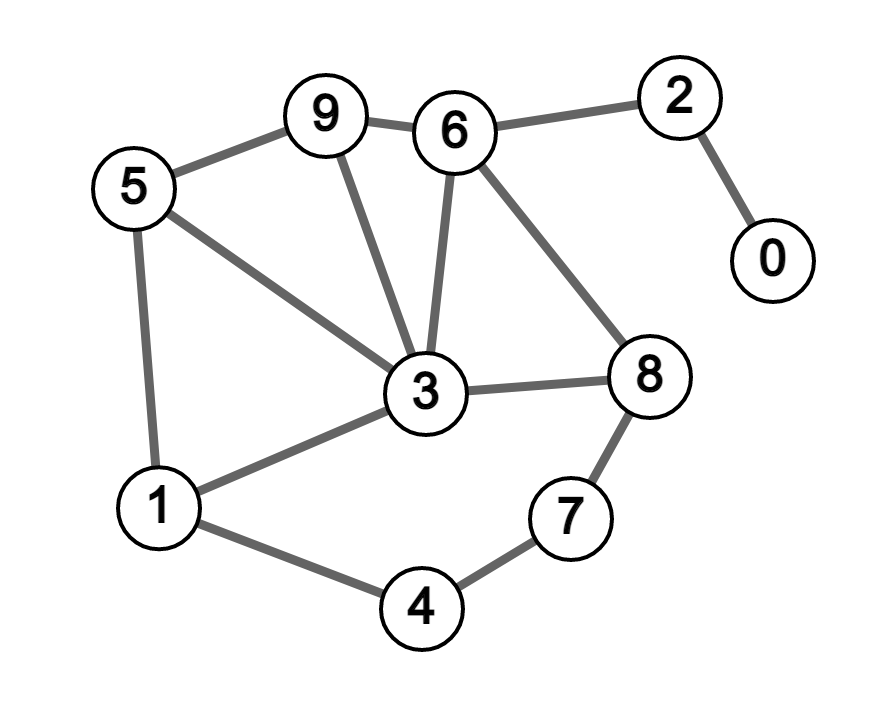
\includegraphics[width=\linewidth]{img/undirected_sample.png}
  \caption{Example of an undirected network.}
  \label{fig:net_un}
\end{figure}

In contrast to that binary relationship of Facebook friendships we have Twitter's system of followers.
Twitter's network can be represented as a directed graph.
The connections between users are directional:
User $A$ can follow user $B$ without the latter following the former.

\begin{figure}[H]
  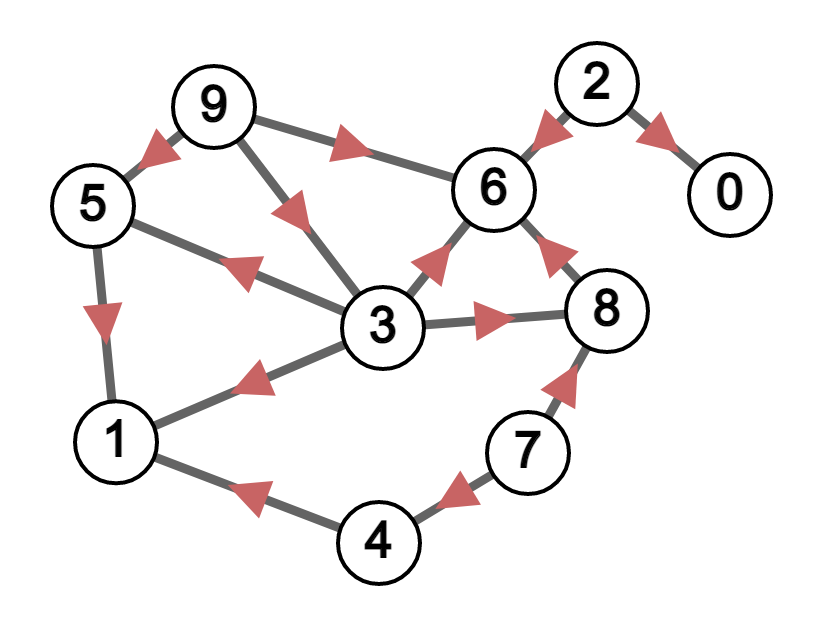
\includegraphics[width=\linewidth]{img/directed_sample.png}
  \caption{Network in previous example with randomized directed edges.}
  \label{fig:net_di}
\end{figure}

The library considers all networks to be weighted on a technical level.
This means that, when created, any edge or vertex has their weight set to one.
An unweighted network is thus just a network with all weights set to the default of one.

Visually, the weight of an edge is usually represented as thickness.
A weighted network could be used to represent interactions between people in a day.
The more interactions users have, the greater the edge's weight.

\begin{figure}[H]
  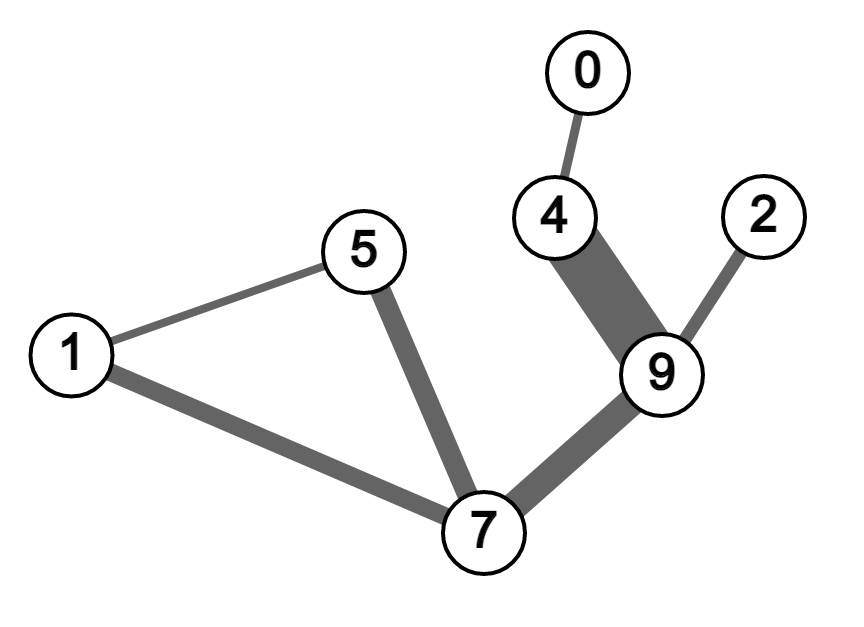
\includegraphics[width=\linewidth]{img/weighted_sample.png}
  \caption{A network with weighted edges.}
  \label{fig:net_weight}
\end{figure}

In Figure \ref{fig:net_weight}, individuals $9$ and $4$
interacted many times during the day, whereas $4$ and $0$
interacted very little. $5$ and $4$ didn't interact at all.